Another quick and easy way to glance at recurrent event data is by event
plots. The \pkg{reReg} provides a convenient way to create event plots
by allowing users to plot the \texttt{Recur} object with the generic
function \texttt{plot()}.

More specifically, the event plot can be stratified by discrete
variables. For example, an event plot stratified by whether the patients
receive chemotherapy (\texttt{chemo\ =\ 1} if no and
\texttt{chemo\ =\ 2} if yes) can be created by the \texttt{plotEvents()}
function with the \texttt{Recur} object as a formula response and
\texttt{chemo} as a covariate.

\begin{figure}[H]
\caption{Event plots}
\begin{center}
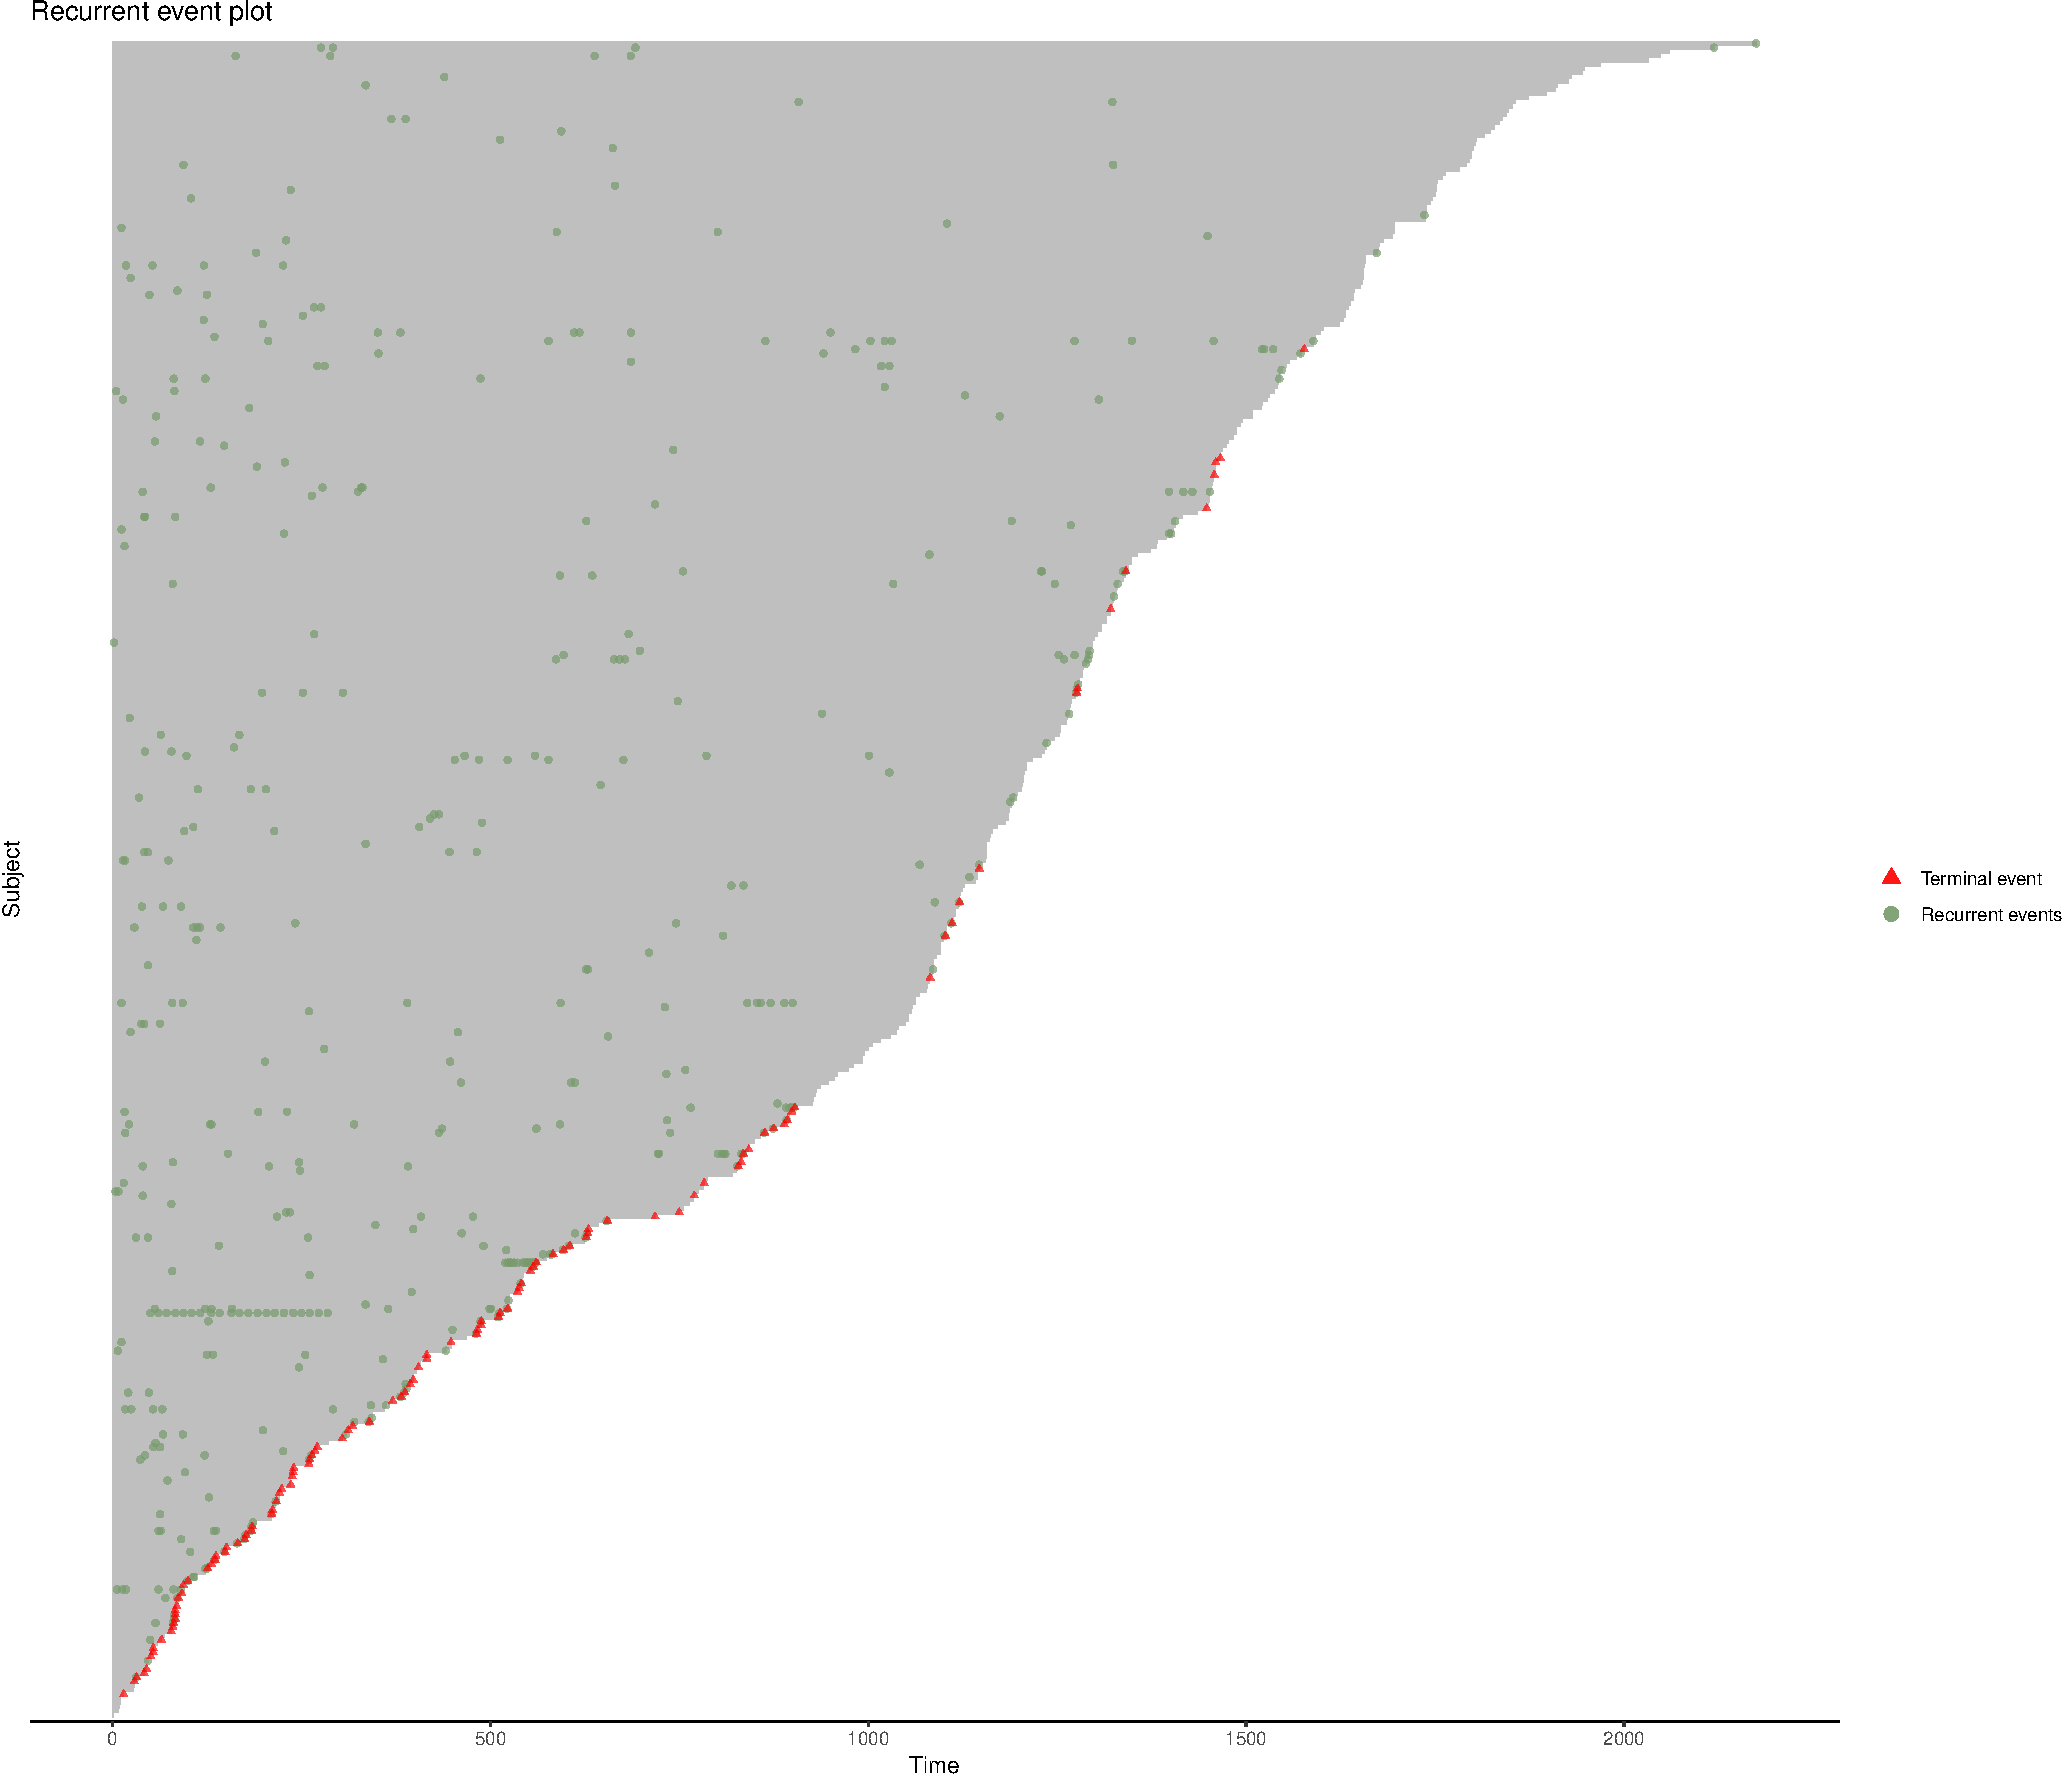
\includegraphics[scale = .125]{images/ep-1}
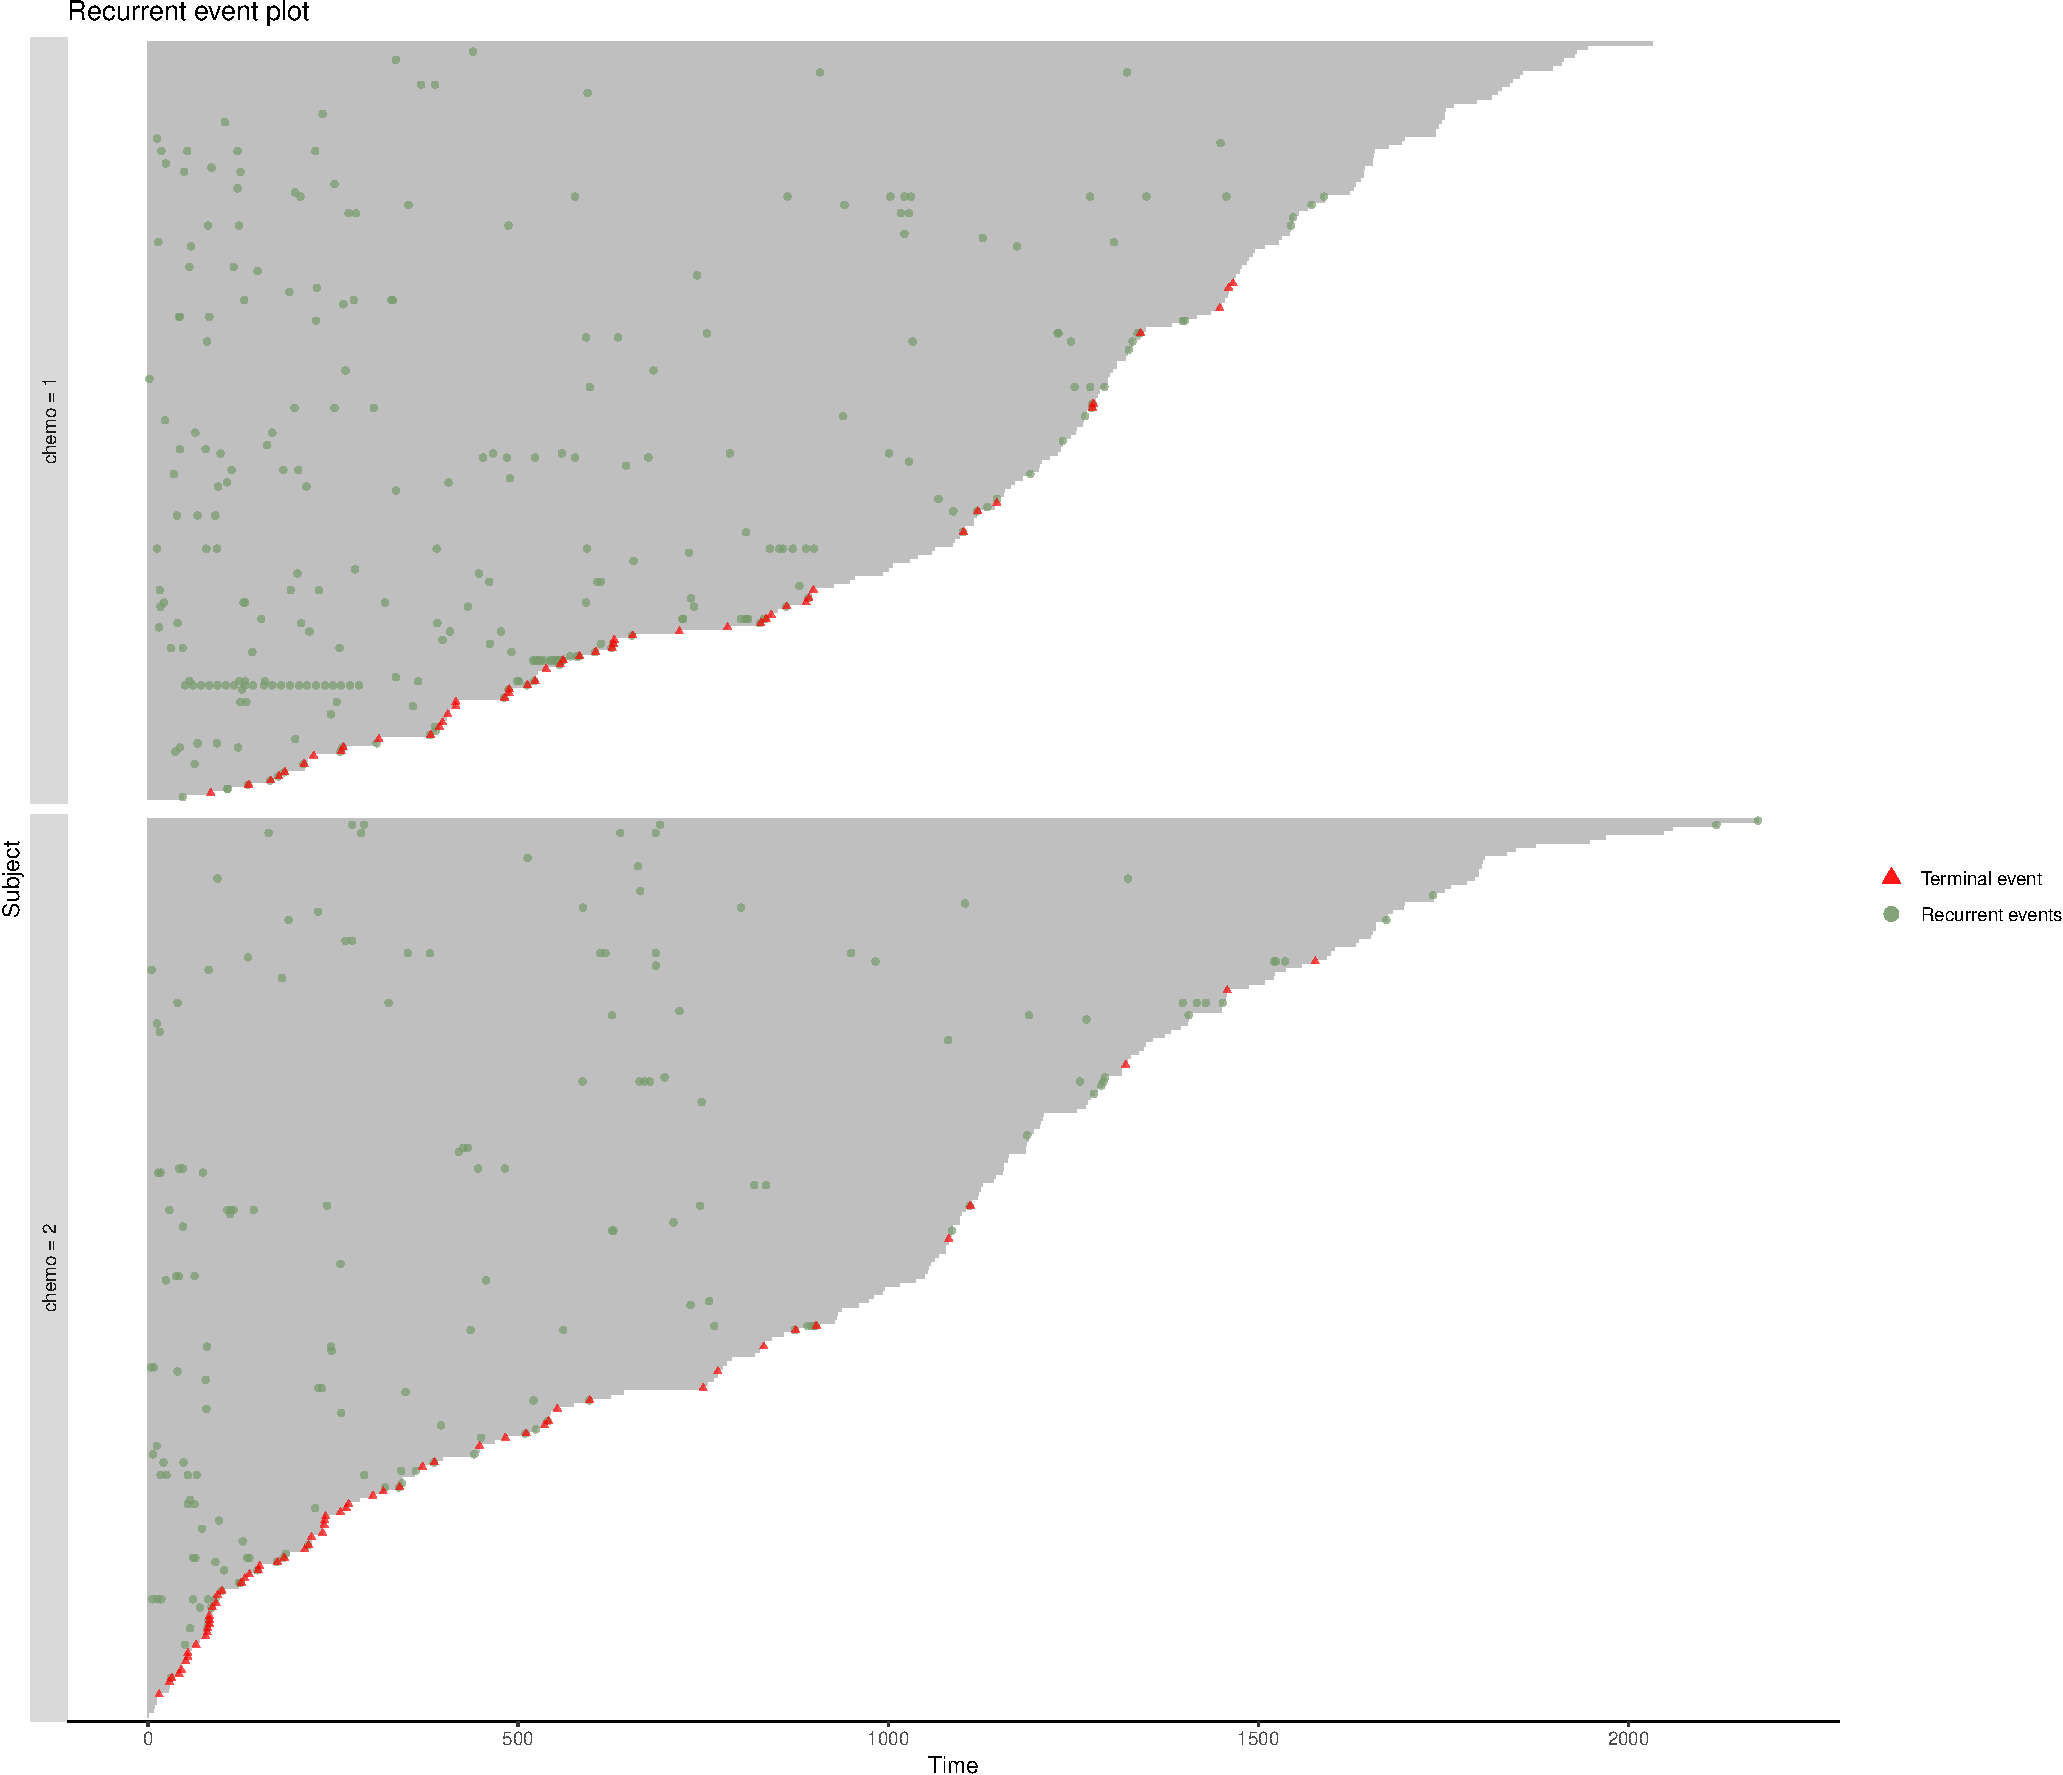
\includegraphics[scale = .125]{images/epChemo-1}
\end{center}
\end{figure}
